\section{Threshold and color space}
\subsection{How did you create the filter? Did you get a good result, i.e. like the middle image of Figure 1? Why/why not? (Possibly there is a lot of white pixels – do not worry).}
By hemming in the colour space of the Red, Green \& Blue bands as little of the desired values were removed. It is not ideal and parts of the scene has parts which contain the RGB spans even if it does not look "green"
\subsection{Suggest how to improve the result.}
By switching from RGB to HSV we could pick out a single colour rather than a span of colour combinations.
\subsection{How do you create the green filter in this color space? Which parameter was the most important?}
Due to there being few items in the scene with similar hues and the bag being fairly uniformly coloured it can easily be cut out and in the HSV view.
\subsection{How does your filtered image compare to the previous RGB-based result?}
Massivly improved and most white specks are removed leaving only the bag.
\subsection{How did you do this?}
We spun the RGB values clockwise within the mask which contained the bag. Turning Red to Green, Green to Blue and Blue to Red. This could have been done in the HSV but the image was already in RGB.
\subsection{Show the resulting image}
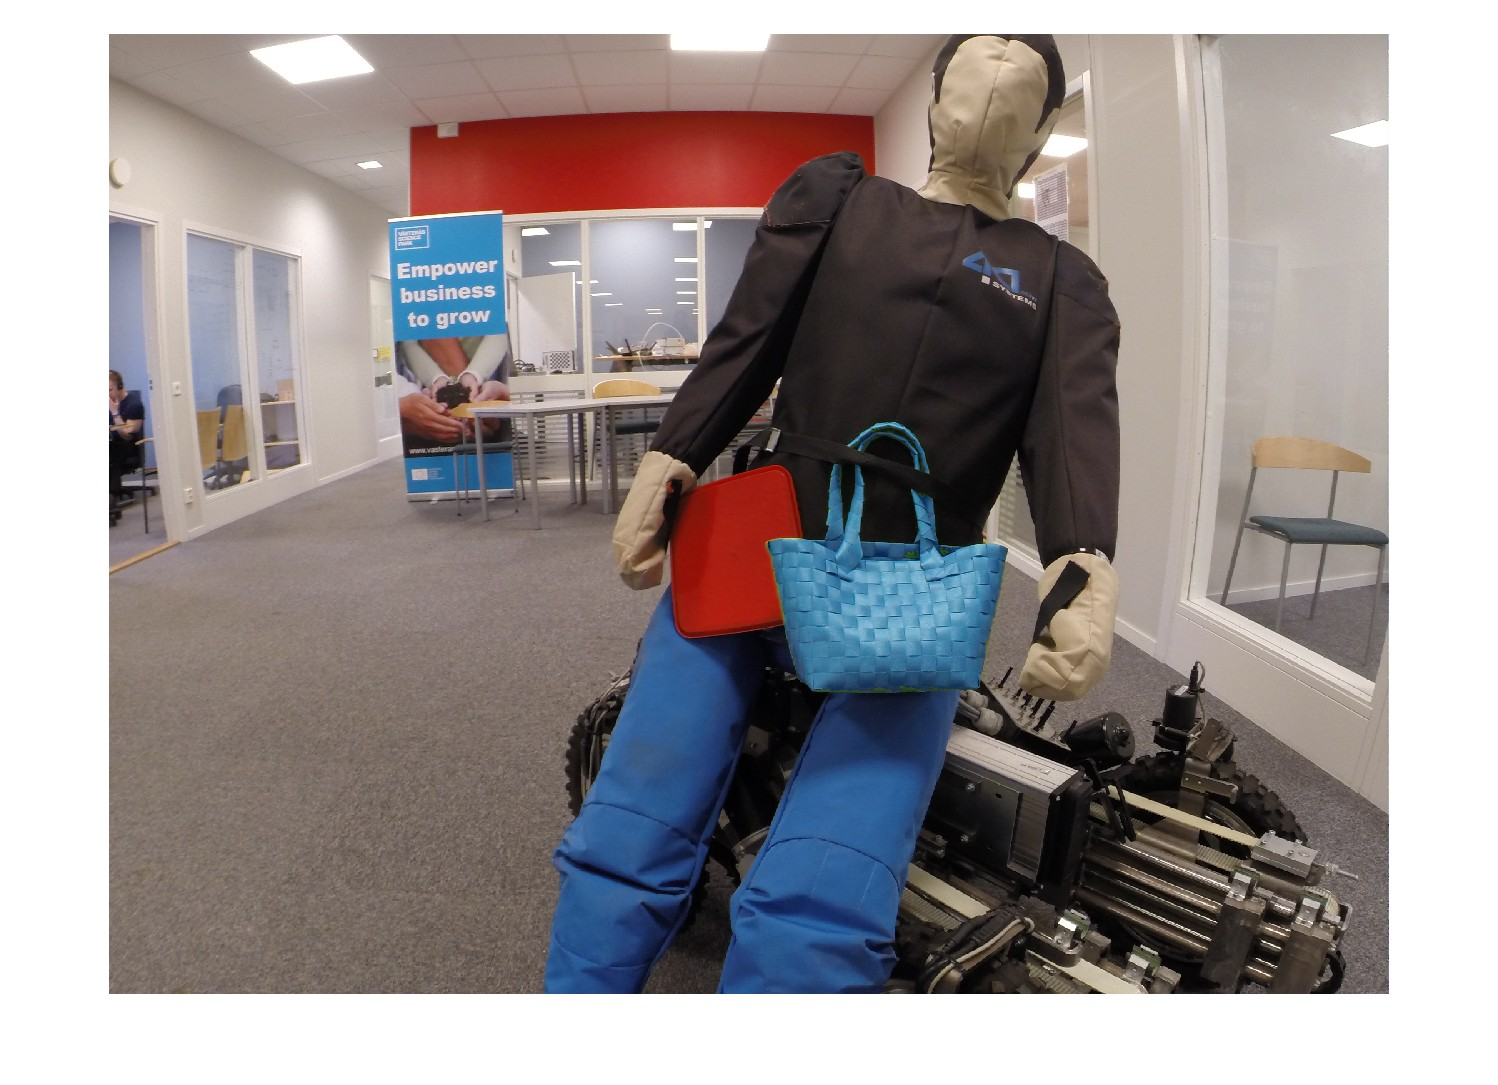
\includegraphics[width=\textwidth]{./bluebag.jpg}
\section{Spatial operator and convolution}
\subsection{Compare A=(I*s)*g and B=I*(s*g). Do they produce the same result?}
Yes.
\subsection{Which one is quicker and why? Use tic, toc. Note: As the image is small loop the operation to get a better time estimation}
A took 0.556078s for 1000 iterations
B took 0.190311s for 1000 iterations
\section{Calibration and measurement}
\subsection{What was the result of your 4 depth estimations? What do you conclude from these with respect to measurement and distortion?}
Disrtorted Pen1 distance was estimated to be 203,0067mm away
Disrtorted Pen2 distance was estimated to be 197,5683mm away
Undisrtorted Pen1 distance was estimated to be 201,4475mm away
Undisrtorted Pen2 distance was estimated to be 202,2000mm away

Human error of picking the pixels are a way larger factor than the undistortion function corrects. The two undistorted distances are closer to eachother and can be assumed to be more accurate. Visually the undistorted images look subjectivly better around the center of the image.
